%!TEX root = thesis.tex


\section{Results}
\subsection{Quantum K-Means}


The algorithm implemented and tested is a variant of the one described in ~\cite{Casper}. The genetic operations of cross-over and mutation are both part of the genetic algorithms toolbox, but were not implemented due to the suggestion from ~\cite{Wiebe2014}. This decision was based on the findings of ~\cite{Liu2010}, stating that the use of the angle-distance rotation method in the quantum rotation operation produces enough variability, with a careful choice of the rotation angle.

\subsubsection{Testing and Results}
The testing was aimed at benchmarking both accuracy and speed. The input used was synthetic data, namely, Gaussian mixtures with variable cardinality and dimensionality. The algorithm was implemented in Python 2.7 and the tests were executed in a machine with an Intel i5 processor, 2GB RAM and running Ubuntu 14.04.

(copy of report)

Regarding the Quantum K-Means (QK-Means), the tests were performed using 10 oracles, a qubit string length of 8 and 100 generations per round. The \textbf{classical} K-Means was executed using the \textbf{k-means++} centroid initialization method, since QK-Means also has some computational cost in the beginning of the algorithm.. Since QK-Means executes a classical K-Means for each oracle each generation, the number of initializations for K-Means was $num.oracles \times num.generations \times factor$, where $factor$ is an adjustable multiplier. Each test had 20 rounds t allow for statistical analysis of the results.

All tests were done with 6 clusters (natural number of clusters). Two tests were done with the two dimensional dataset: one with a $factor=1.10$ (increase initializations by $10\%$) and another with $factor=1$. These tests will be called T1 and T2, respectively. The test done with the six dimensional dataset (T3) used $factor=1.10$.

Timing results

% table in csv format available in resource directory -->

\begin{table}[h]
\caption{Timing results for the different algorithms in the different tests. Fitness time refers to the time that took to compute the DB index of each solution of classical K-Means. All time values are the average over 20 rounds and are displayed in seconds.}
\begin{tabular}{|l|l|l|l|l|l|}
\hline
\textbf{Dataset}               & \textbf{Algorithm} & \textbf{Mean} & \textbf{Variance} & \textbf{Best} & \textbf{Worst} \\ \hline
\textbf{T1}                    & QK-Means           & 62.02642975   & 0.077065212       & 61.620424     & 62.579969      \\ \cline{2-6} 
\textbf{bi36}                  & K-Means            & 6.4774672     & 0.002501651       & 6.352554      & 6.585451       \\ \cline{2-6} 
\textbf{}                      & K-Means + fitness  & 70.2238286    & 0.022223755       & 69.889105     & 70.548572      \\ \cline{2-6} 
\textbf{}                      & fitness            & 63.7463614    & 0.019722105       & 63.536551     & 63.963121      \\ \hline
\textbf{T2}                    & QK-Means           & 64.22347165   & 0.056559152       & 63.807367     & 64.807373      \\ \cline{2-6} 
\textbf{bi36 noFactor} & K-Means            & 5.71167475    & 0.004903253       & 5.581391      & 5.877091       \\ \cline{2-6} 
\textbf{}                      & K-Means + fitness  & 62.7021533    & 0.066919692       & 63.417207     & 62.180021      \\ \cline{2-6} 
\textbf{}                      & fitness            & 56.99047855   & 0.062016439       & 56.59863      & 57.540116      \\ \hline
\textbf{T3}                    & QK-Means           & 74.4917966    & 0.067688312       & 74.12105      & 74.976446      \\ \cline{2-6} 
\textbf{sex36}                 & K-Means            & 8.291648      & 0.007015777       & 8.160859      & 8.426203       \\ \cline{2-6} 
                               & K-Means + fitness  & 72.36315915   & 0.05727269        & 71.856457     & 73.031841      \\ \cline{2-6} 
                               & fitness            & 64.07151115   & 0.050256913       & 63.695598     & 64.605638      \\ \hline
\end{tabular}
\end{table}

The mean computation time of classical K-Means is an order of magnitude lower than that of QK-Means. However, in classical K-Means the solution typically chosen is the one with lowest sum of squared euclidean distances of points to their attributed centroid. To make a fair comparison between the two algorithms, the Davies-Bouldin index of all classical K-Means solutions was computed and used as the criteria to choose the best solution. When this is done, we can see that the total time of classical K-Means is actually higher that that of QK-Means in T1 and T3, but this is only due to the 1.10 multiplier on the number of initializations. In T2, possibly the fairest comparison, the computation times become very similar with only a 2\% difference between the two algorithms.

Accuracy

Comparing K-Means and QK-Means

% table in csv format available in resource directory -->

\begin{table}[h]
\caption{All values displayed are the average over 20 rounds, except for the Overall best which shows the best result in any round. The values represent the Davies-Bouldin fitness index (low is better).}
\begin{tabular}{|l|l|l|l|l|l|l|}
\hline
\textbf{Dataset} & \textbf{Algorithm} & \textbf{Best} & \textbf{Worst} & \textbf{Mean} & \textbf{Variance} & \textbf{Overall best} \\ \hline
\textbf{T1}      & QK-Means           & 15.42531927   & 32.29577426    & 19.94704511   & 21.23544567       & 15.42531927           \\ \cline{2-7} 
\textbf{}        & K-Means            & 15.42531927   & 25.44913817    & 16.25013365   & 1.216919278       & 15.42531927           \\ \hline
\textbf{T3}      & QK-Means           & 22.72836641   & 65.19984617    & 36.10699242   & 78.14043743       & 22.71934191           \\ \cline{2-7} 
\textbf{}        & K-Means            & 22.71934191   & 46.72231967    & 26.18440481   & 22.96730826       & 22.71934191           \\ \hline
\end{tabular}
\end{table}

The most relevant result in the table above is the mean of the best index. The value is the average over all rounds of the best solution in each round and it provides insight on the average performance of the algorithm. The results suggest that both algorithms perform equally well. The best overall result of each algorithm in all rounds is exactly the same. In T3, the mean performance of classical K-Means is marginally better.

I speculate that if classical K-Means was using only the sum of euclidean distances and not the DB index, the average performance would be worse. As it stands, choosing to use DB index with classical K-Means possibly represents a tradeoff between speed and accuracy.

QK-Means details

Here we’ll analyse a bit what’s happening within each QK-Means execution. One would expect for the population’s fitness variance to decrease over the generations, as the probabilities for previous known solutions increase and are therefore more likely to reappear. The convergence of the population mean would also be expected to decrease for the same reason. However, experimental (Fig. \ref{fig:db_index_mean_t2} and \ref{fig:db_index_var_t2}) results don’t suggest any of these expectations (the results of T1 and T3 suggest the same). This may be due to low number of generations or simply because the random generation of initial centroids isn’t influenced enough by the qubit probabilities.


\begin{figure}[hbtp]
\centering
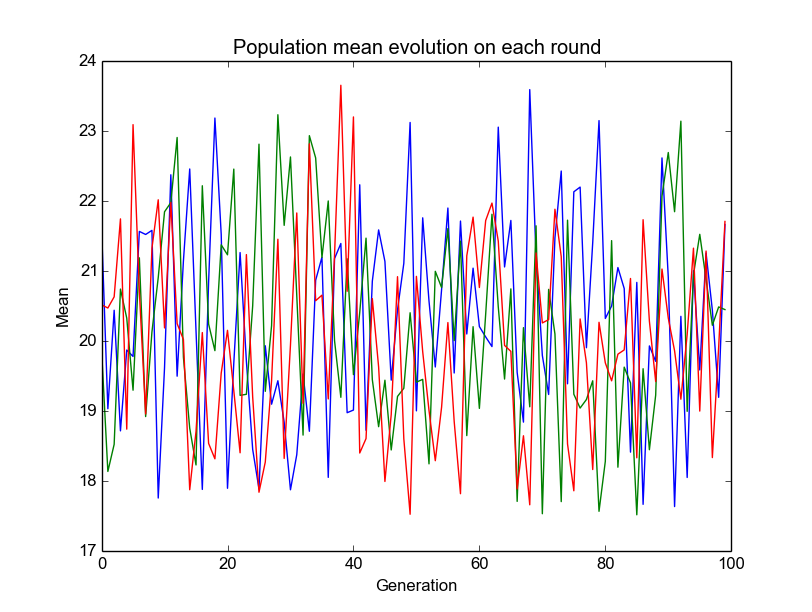
\includegraphics[scale=0.5]{QK_Means/img/bi_nofactor_mean.png}
\caption{DB index mean of the population in T2. Only 4 rounds represented.}
\label{fig:db_index_mean_t2}
\end{figure}

\begin{figure}[hbtp]
\centering
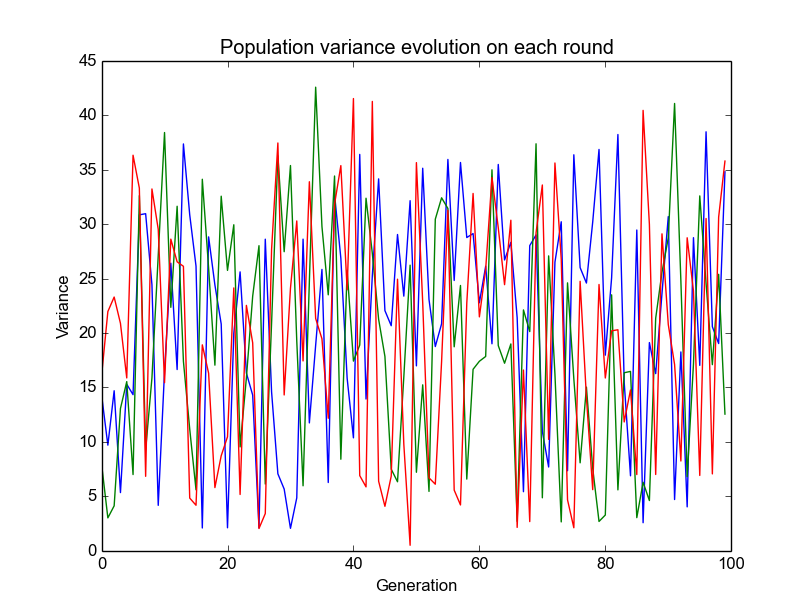
\includegraphics[scale=0.5]{QK_Means/img/bi_nofactor_var.png}
\caption{DB index variance of the population in T2. Only 4 rounds represented.}
\label{fig:db_index_var_t2}
\end{figure}


Analysing the evolution of the DB index of the best solution over the generations (Fig. \ref{fig:qk_db_index_best_evo_t2} and \ref{fig:qk_db_index_best_evo_t3}) gives some insight on the rate of convergence. In both tests it is clear that the best solution is often reached in a quarter of the total generations. More detail can be seen in the Table \ref{tab:db_index_t1_t3}.

\begin{figure}[hbtp]
\centering
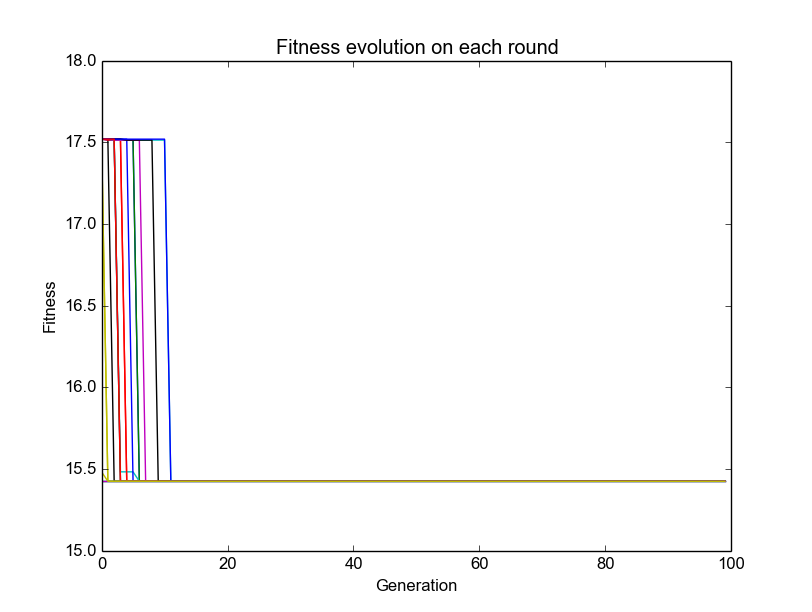
\includegraphics[scale=0.5]{QK_Means/img/bi_nofactor_evo.png}
\caption{DB index of best solution in T2.}
\label{fig:qk_db_index_best_evo_t2}
\end{figure}


\begin{figure}[hbtp]
\centering
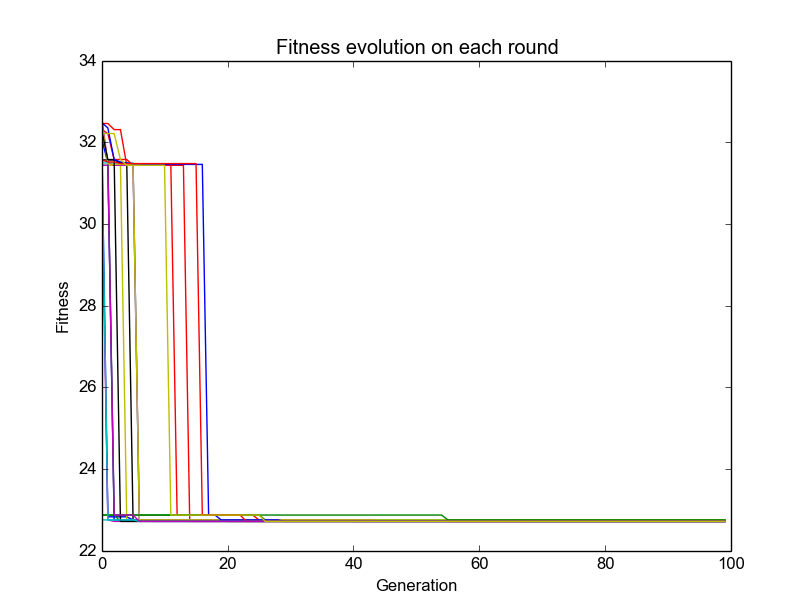
\includegraphics[scale=0.5]{QK_Means/img/sex_evo.png}
\caption{DB index of best solution in T3.}
\label{fig:qk_db_index_best_evo_t3}
\end{figure}

% table in csv format available in resource directory -->

\begin{table}[h]
\caption{The values represent generations.}
\begin{tabular}{|l|l|l|l|l|}
\hline
\textbf{Test} & \textbf{Mean} & \textbf{Variance} & \textbf{Best} & \textbf{Worst} \\ \hline
\textbf{T1}   & 17.25         & 70.2875           & 3             & 33             \\ \hline
\textbf{T3}   & 28.05         & 568.6475          & 2             & 90             \\ \hline
\end{tabular}
\label{tab:db_index_t1_t3}
\end{table}

\subsubsection{Discussion}

Results show that most computational cost (90\% on T1) lies on the evaluation of the solutions obtained from each oracle. This is a costly but necessary step in this algorithm. Moreover, and even though EAC doesn't require its input partitions to be accurate, the quality of the solutions, measured with the Davies-Bouldin index, from QK-Means doesn't differ from that of K-Means. This two facts make the use of this algorithm in EAC prohibitive, as no benefits in compuational time are gained.

It should be noted that the target application of the tests presented differs from that of the original authors and although no accuracy gains were observed in these results, the results might differ on different applications.

\subsection{Horn and Gottlieb's algorithm}


\subsubsection{Testing and Results}


%TODO
%Put in accuracy results for crab,iris and gaussian mixtures  
%Put in timing results


The accuracy of this algorithm was tested with real world datasets, namely, the crab and iris datasets available at the UCI Machine Learning Repository.

%TODO add ref for repository -->

\subsubsection{Iris data}
\label{sec:horn_iris}
The iris dataset ([available at the UCI ML repository](http://archive.ics.uci.edu/ml/datasets/Iris)) has 3 classes each with 50 data points. There are 4 features. The data is preprocessed using Principal Component Analysis (PCA). The natural clustering can be observed in Fig. \ref{fig:iris_natural}. 

% #TODO saved image from ipython -->

\begin{figure}[hbtp]
\centering
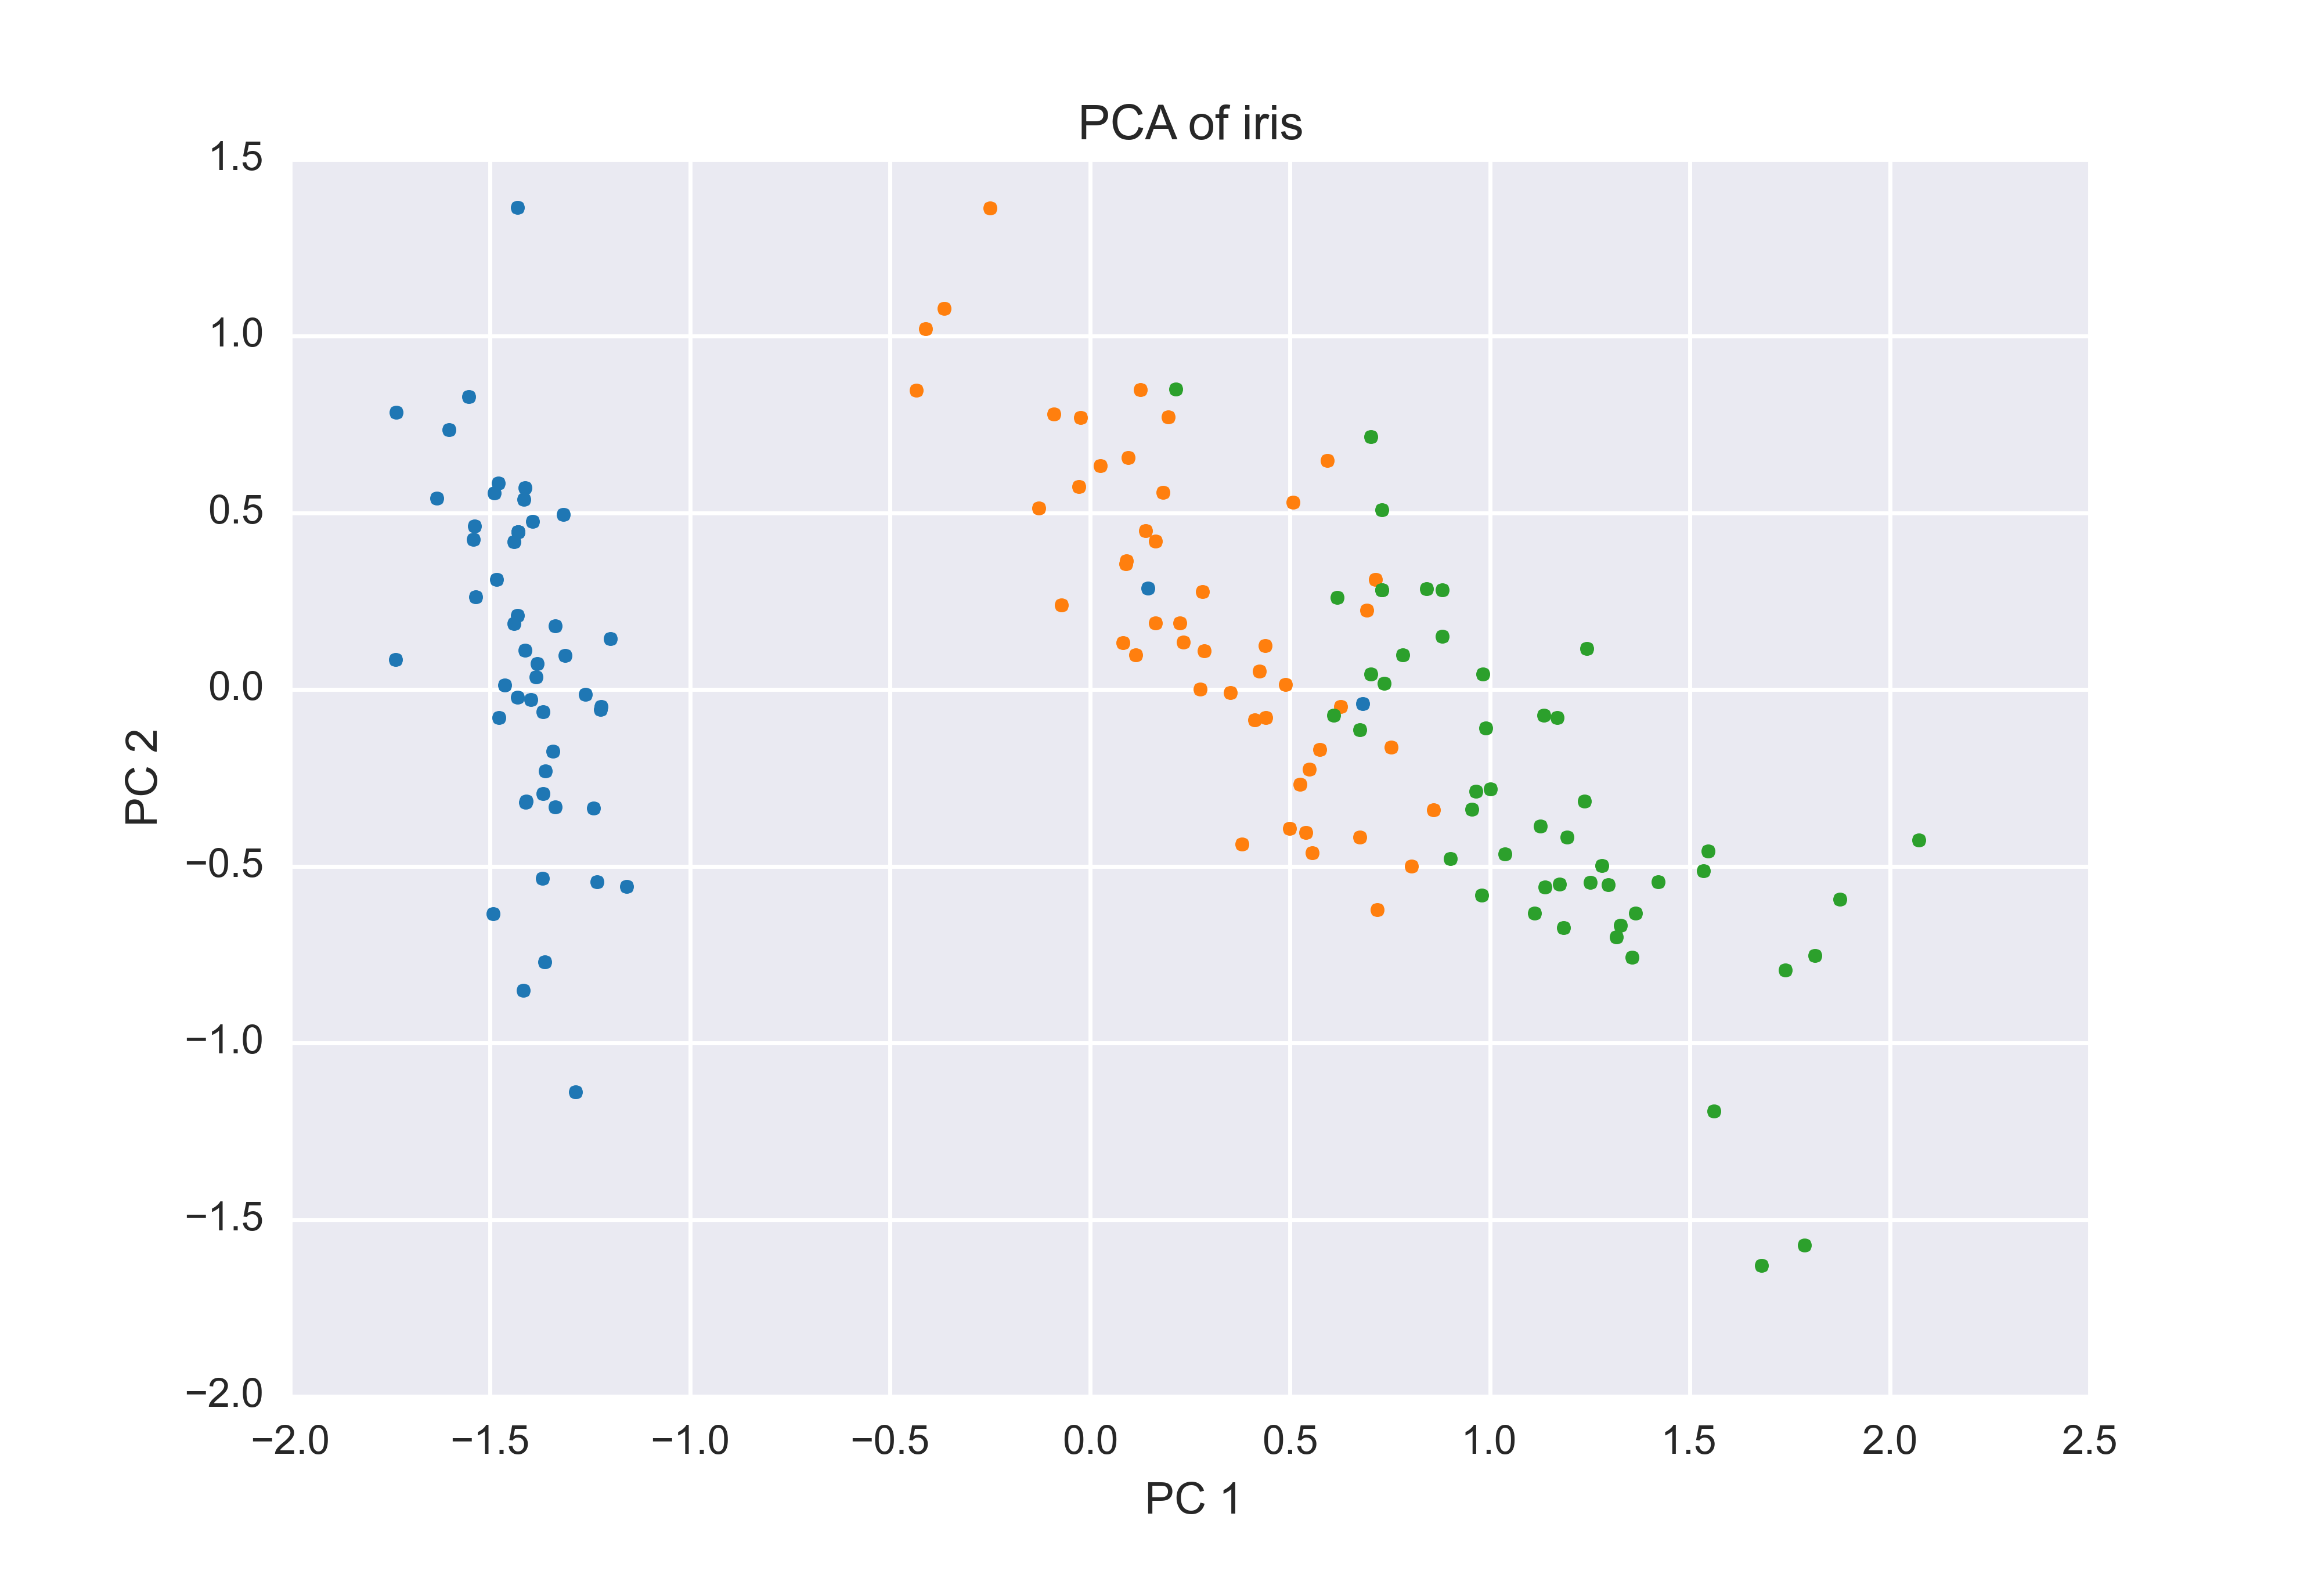
\includegraphics[scale=0.5]{Horn/img/iris_natural.png}
\caption{Plot of the two first principal components (PC).}
\label{fig:iris_natural}

\end{figure}

I chose $\sigma=\frac{1}{4}$ to reproduce the experiments in [3]. Only the first two PC are used here, which account for $95.8\%$ of the energy. The clustering results can be seen in Fig. \ref{fig:iris_2pc_cluster} and have an accuracy of 86\% computed with consistency index.


\begin{figure}[hbtp]
\centering
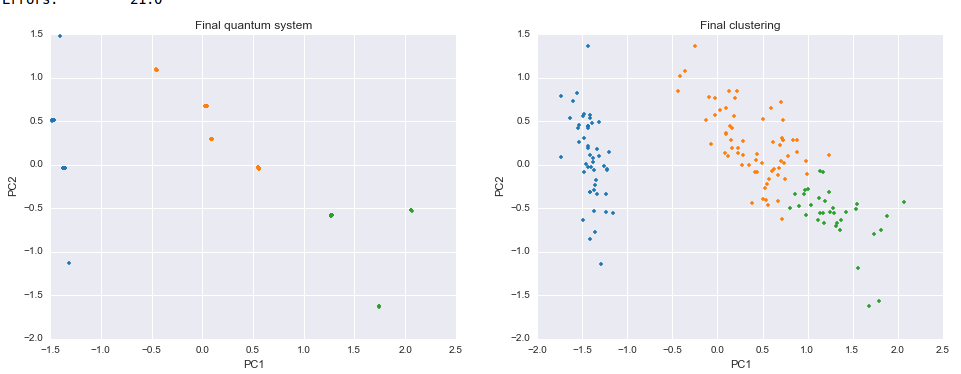
\includegraphics[width=\textwidth]{Horn/img/iris_2pc_cluster.png}
\caption{Plots of the converged data data points and final clustering for 2 PC.}
\label{fig:iris_2pc_cluster}

\end{figure}

For the sake of completeness, Fig. \ref{fig:iris_allpc_cluster} shows the clustering over all PCs. This solution has an accuracy of 82.67\% computed with consistency index.


\begin{figure}[hbtp]
\centering
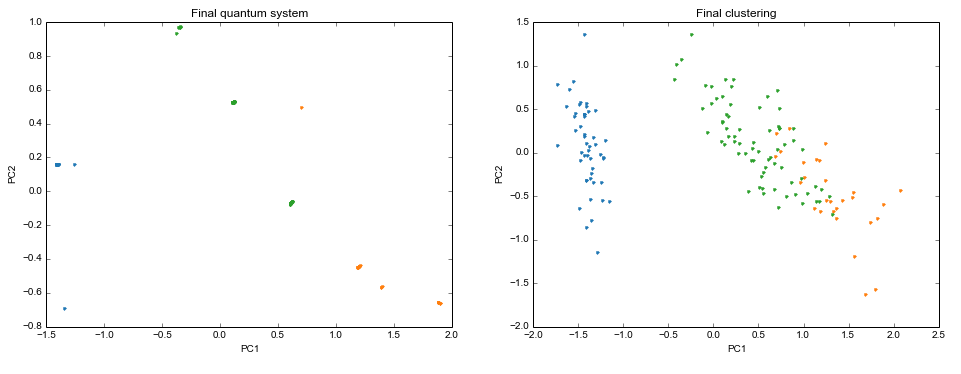
\includegraphics[width=\textwidth]{Horn/img/iris_allpc_cluster.png}
\caption{Plots of the converged data data points and final clustering for all PC of Iris data.}
\label{fig:iris_allpc_cluster}
\end{figure}


\subsubsection{Crab data}


The crabs dataset has 200 samples and describes 5 morphological measurements on 50 crabs each of two colour forms and both sexes (total of 200 crabs), of the species Leptograpsus variegatus collected at Fremantle, Western Australia. After a preprocessing using PCA with covariance matrix and uncentred data, the dataset is represented in Fig. \ref{fig:crab_2pc_covar}.% #TODO add reference to dataset -->

\begin{figure}[hbtp]
\centering
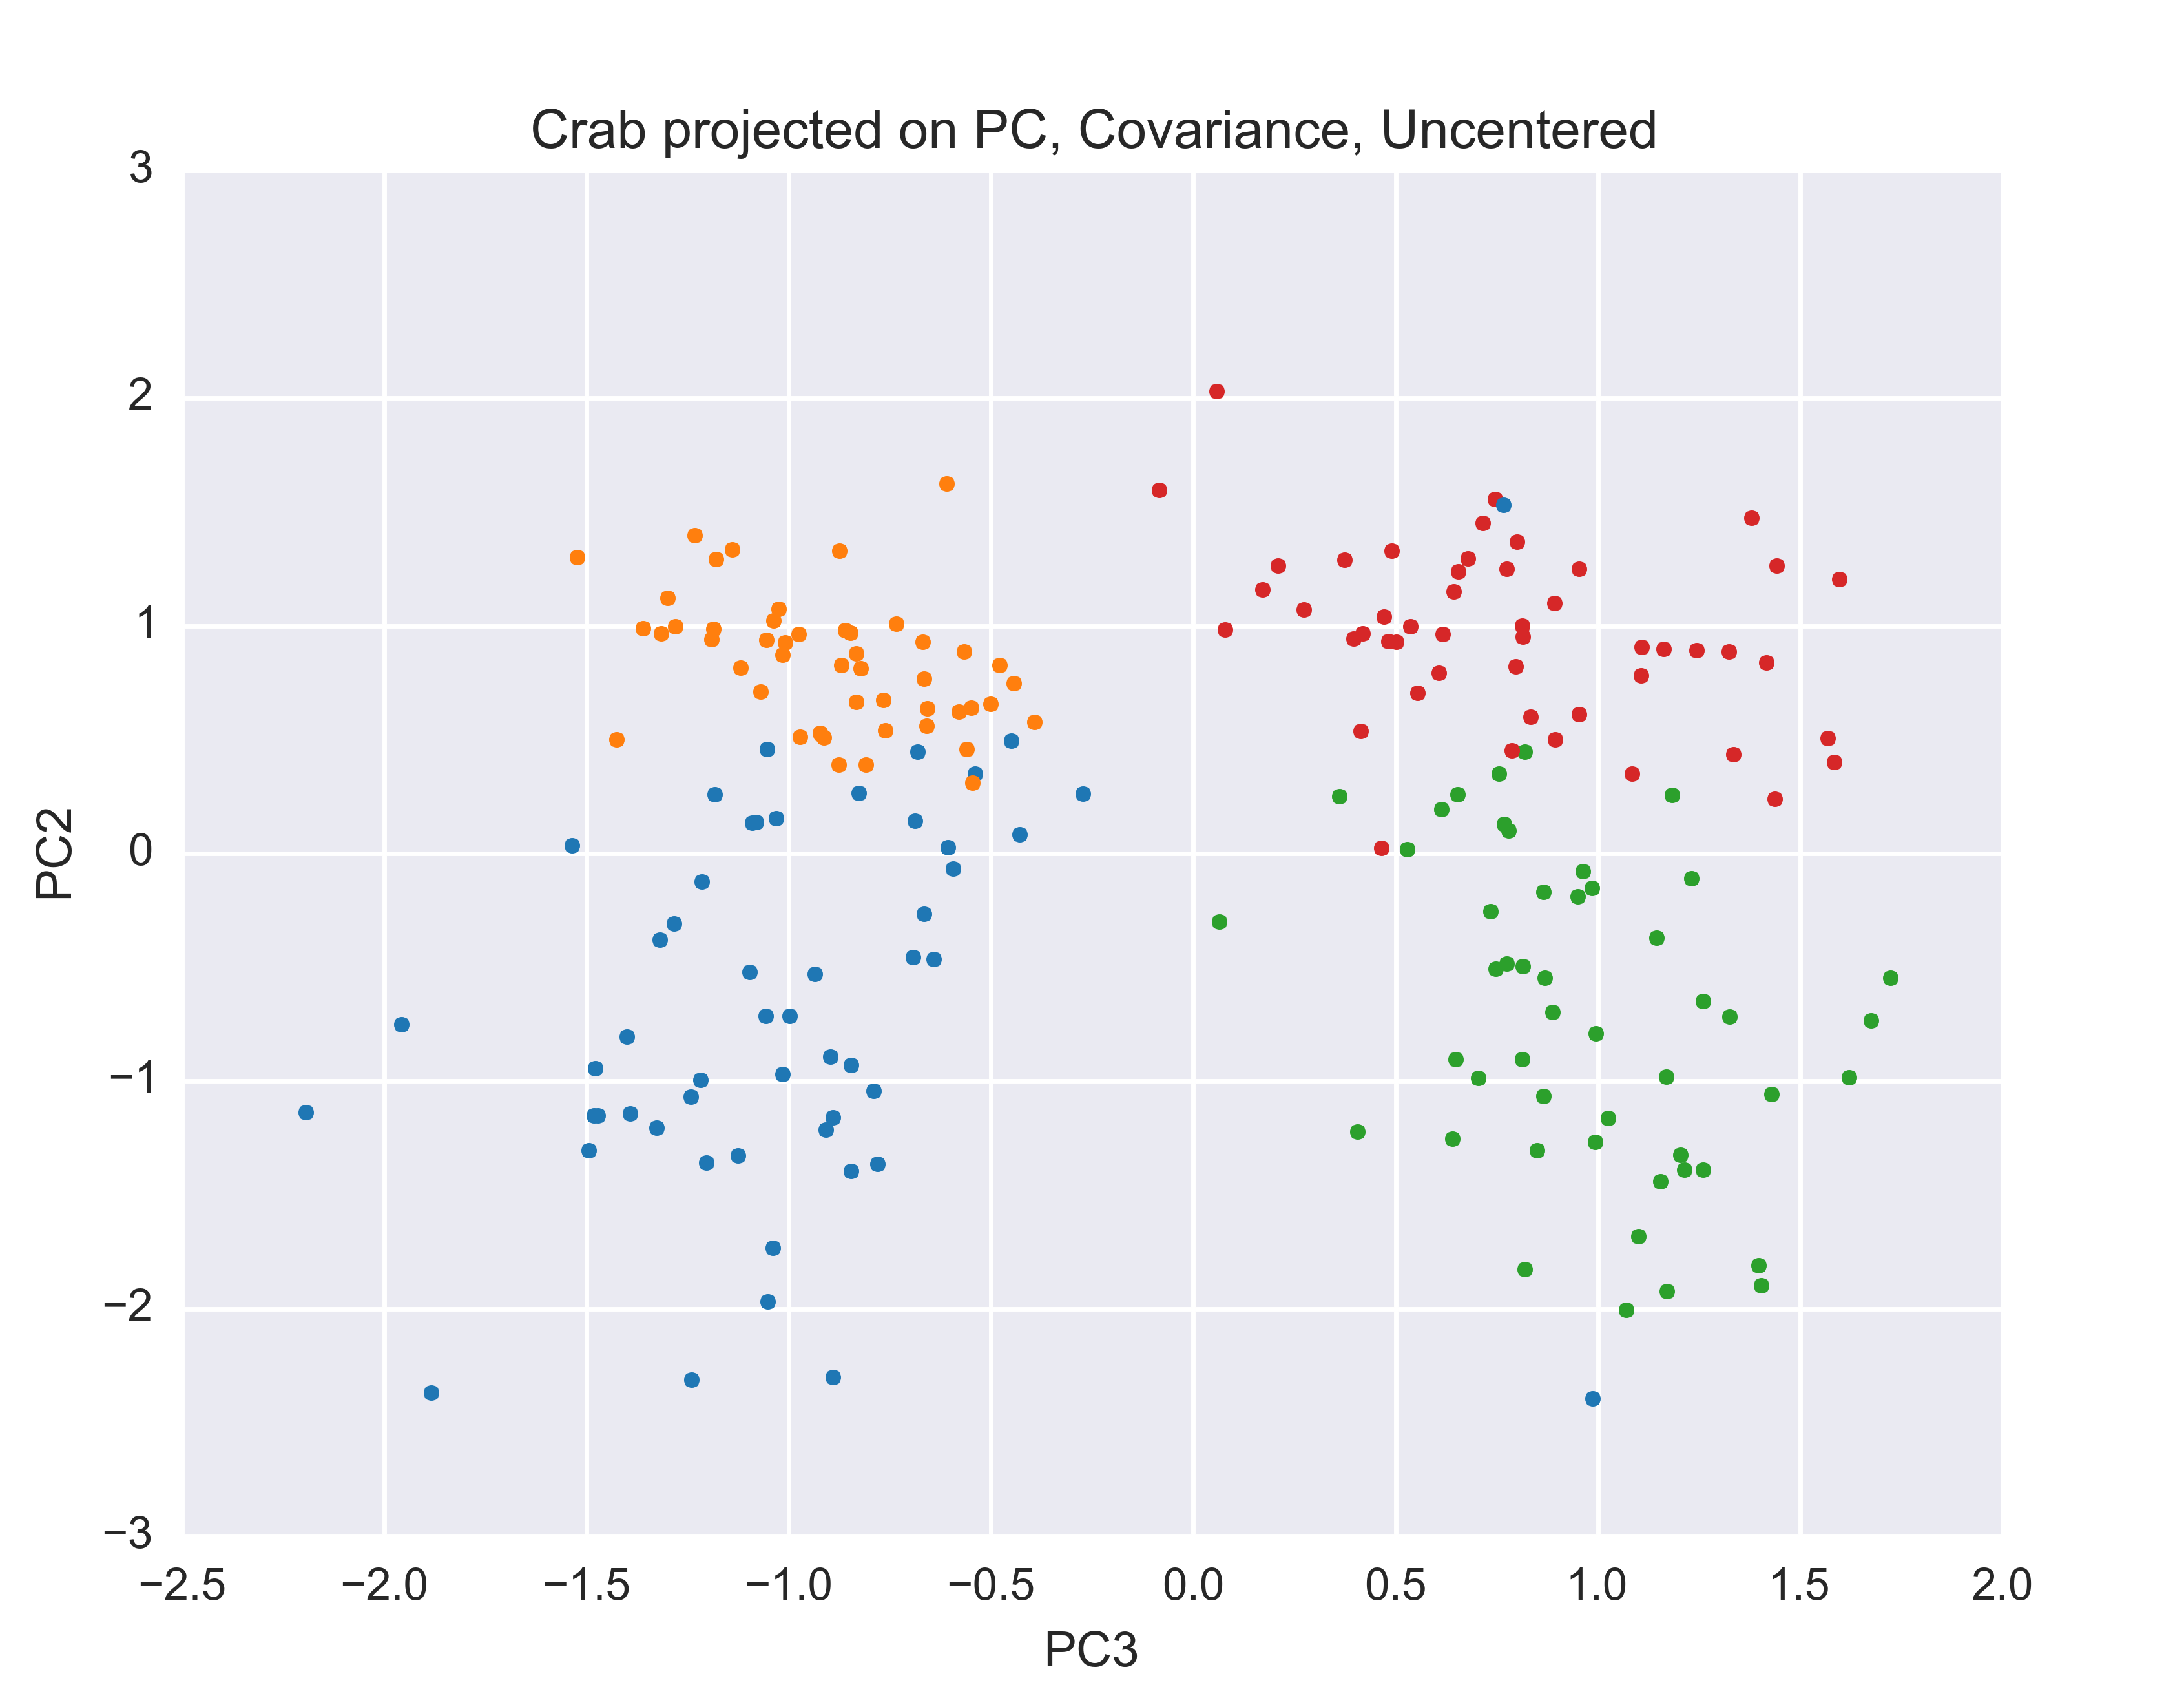
\includegraphics[scale=0.5]{Horn/img/crab_2pc_covar.png}
\caption{Representation of the crab data projected over PC 2 and 3.}
\label{fig:crab_2pc_covar}
\end{figure}

\begin{figure}[hbtp]
\centering
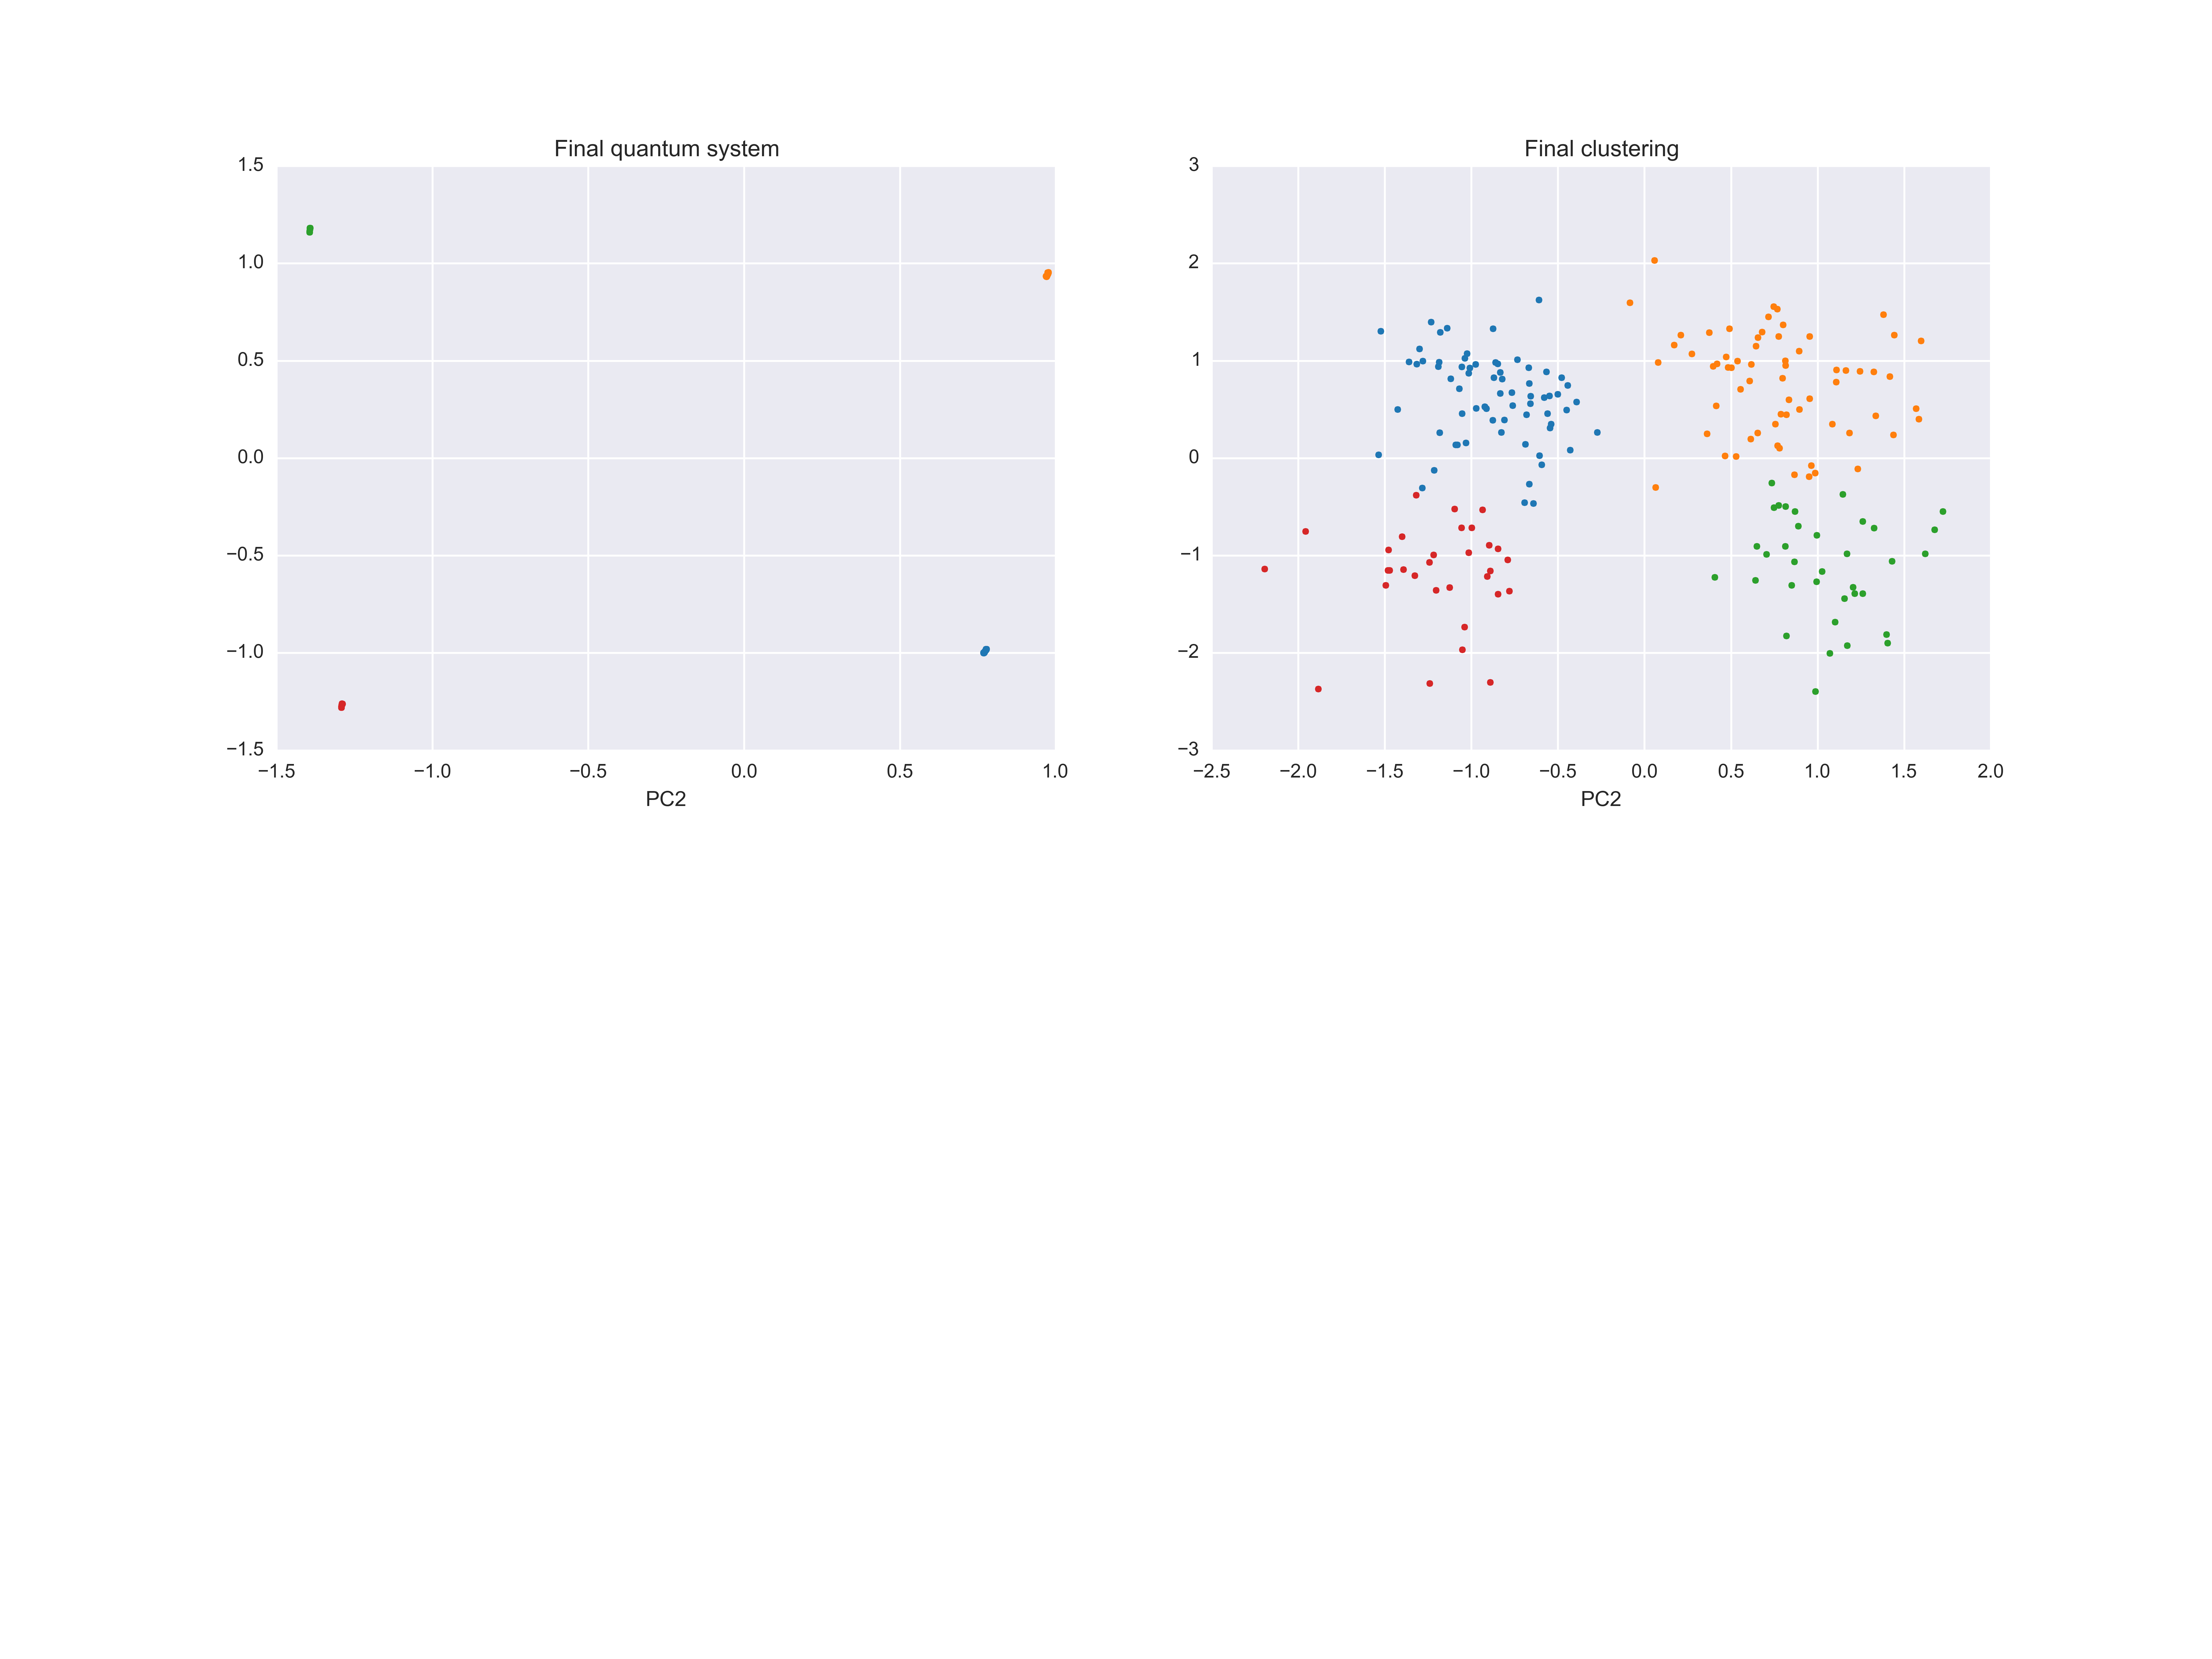
\includegraphics[width=\textwidth]{Horn/img/crab_2pc_covar_cluster.png}
\caption{Representation of the crab data projected over PC 2 and 3.}
\label{fig:crab_2pc_covar_cluster}
\end{figure}

\begin{figure}[hbtp]
\centering
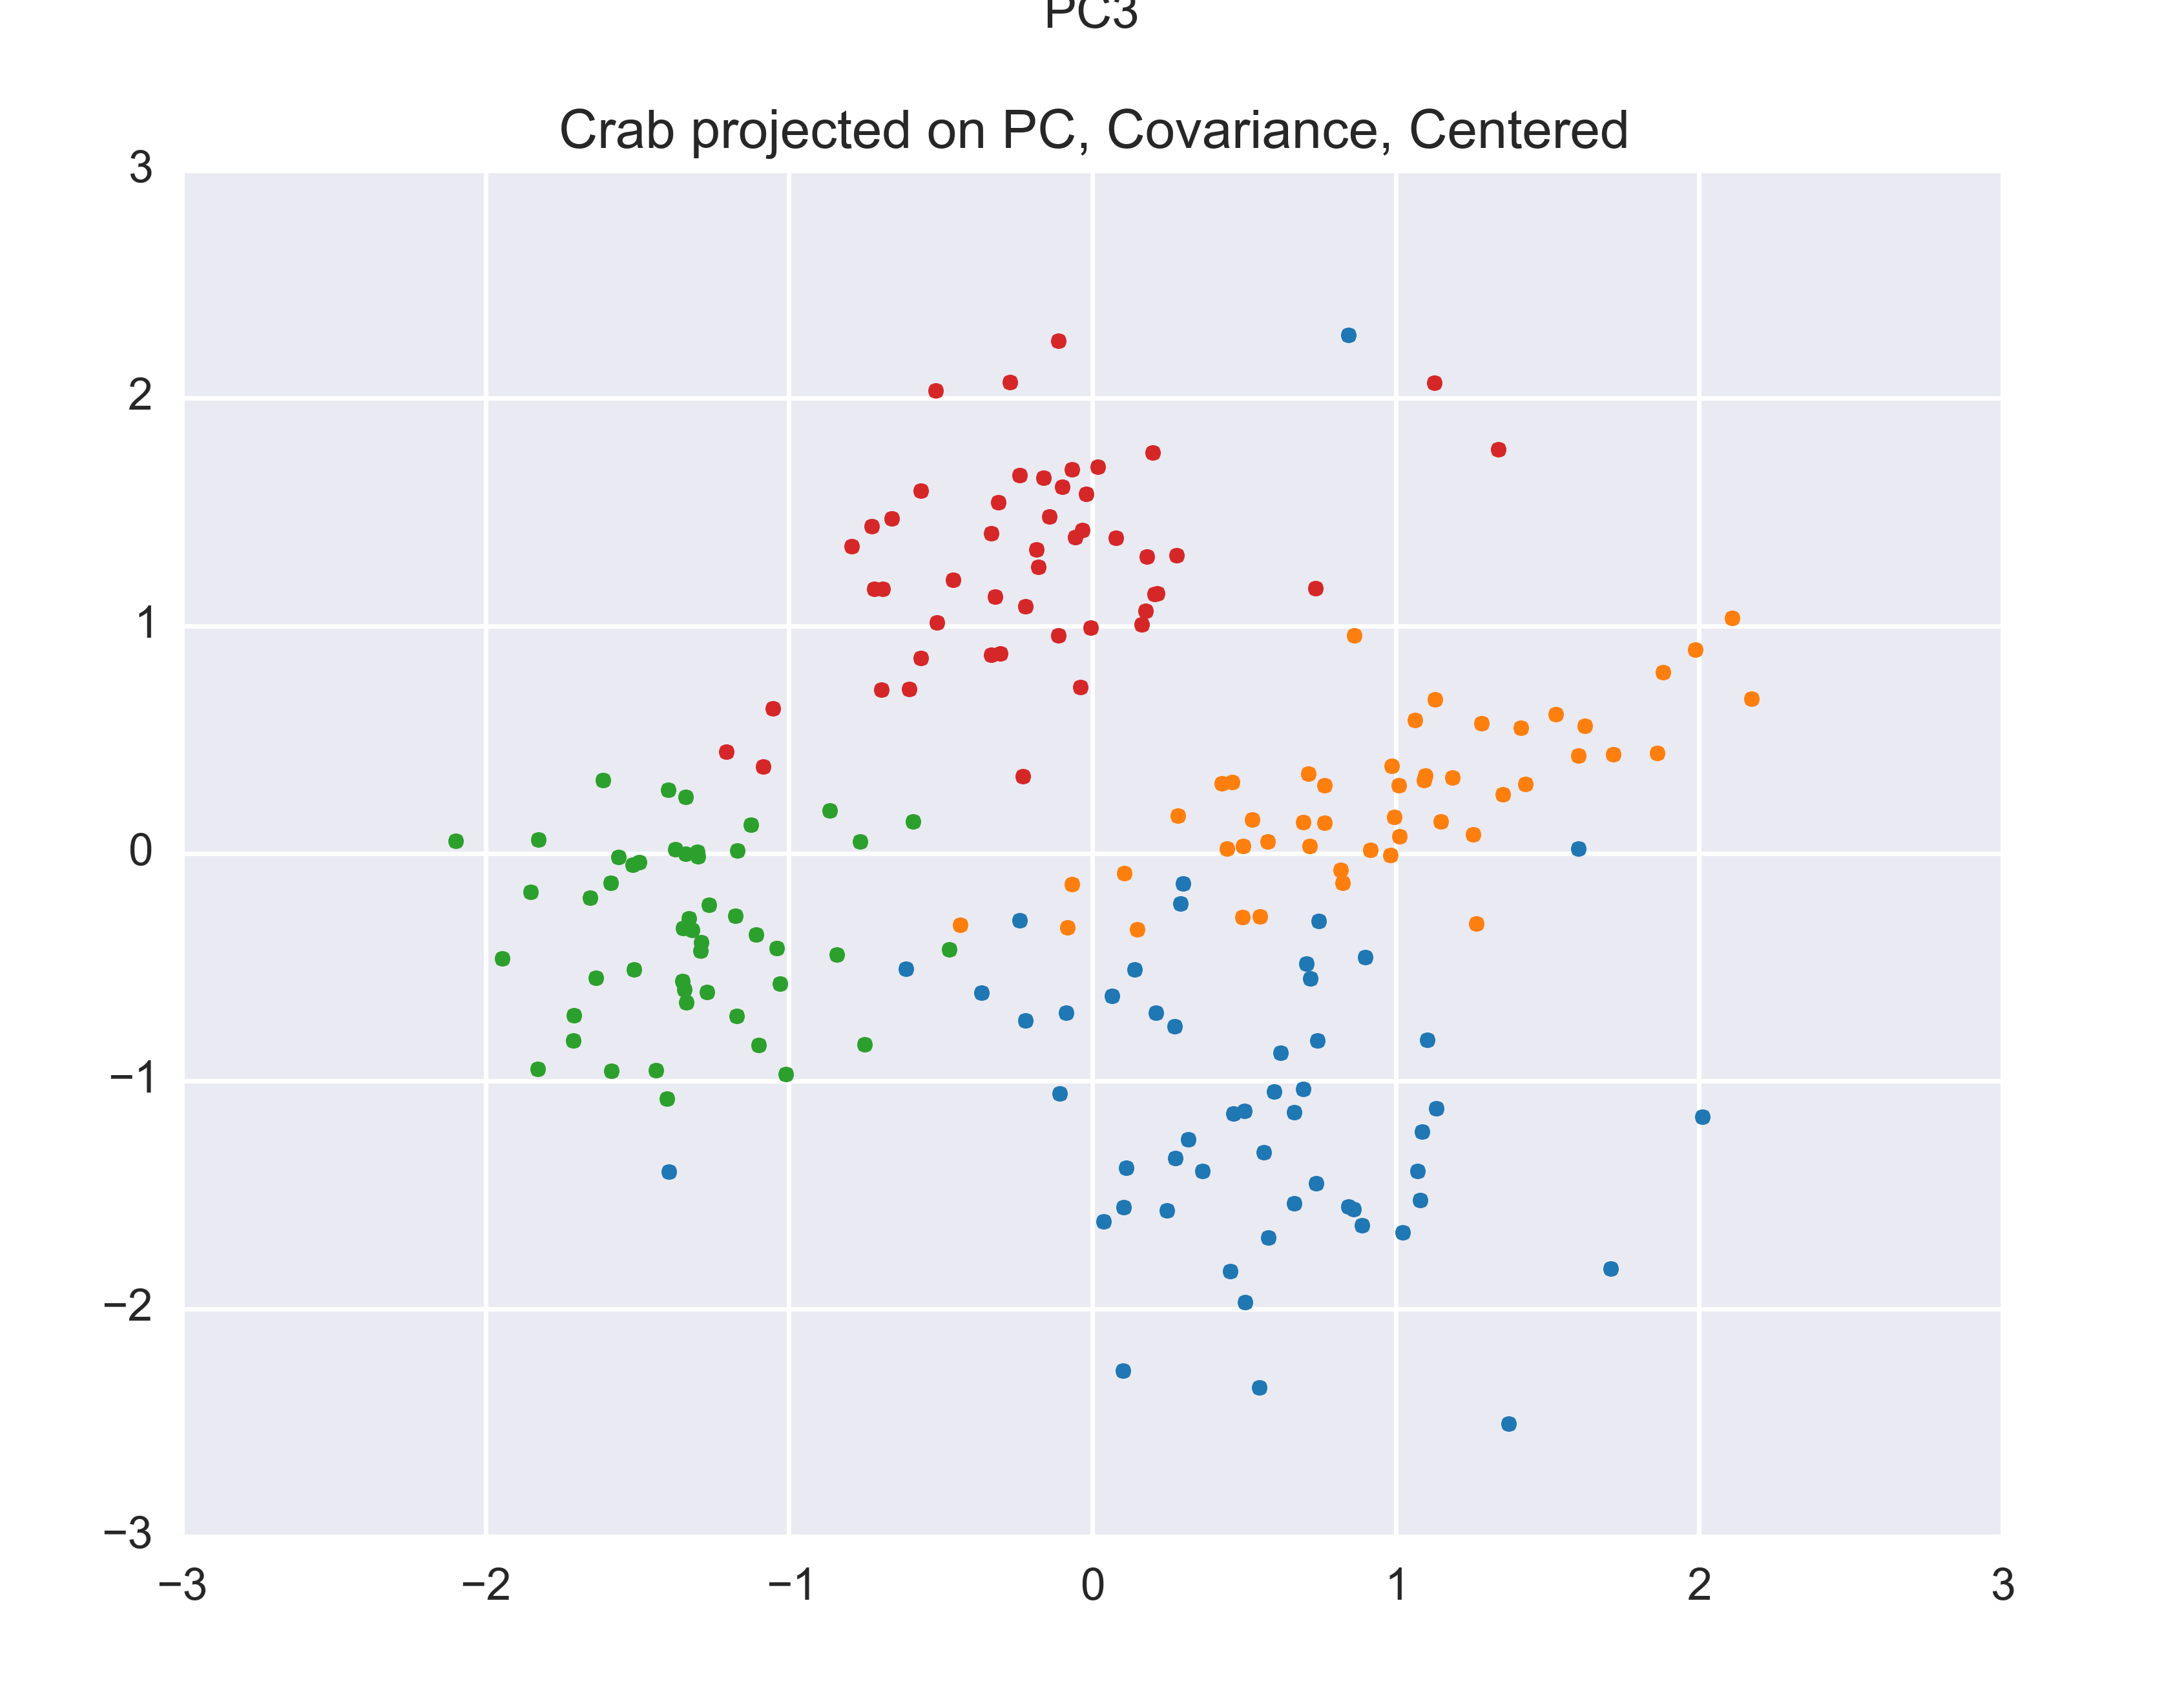
\includegraphics[scale=0.5]{Horn/img/crab_2pc_covar_centered.png}
\caption{Representation of the crab data projected over PC 2 and 3.}
\label{fig:crab_2pc_covar_centered}
\end{figure}

\begin{figure}[hbtp]
\centering
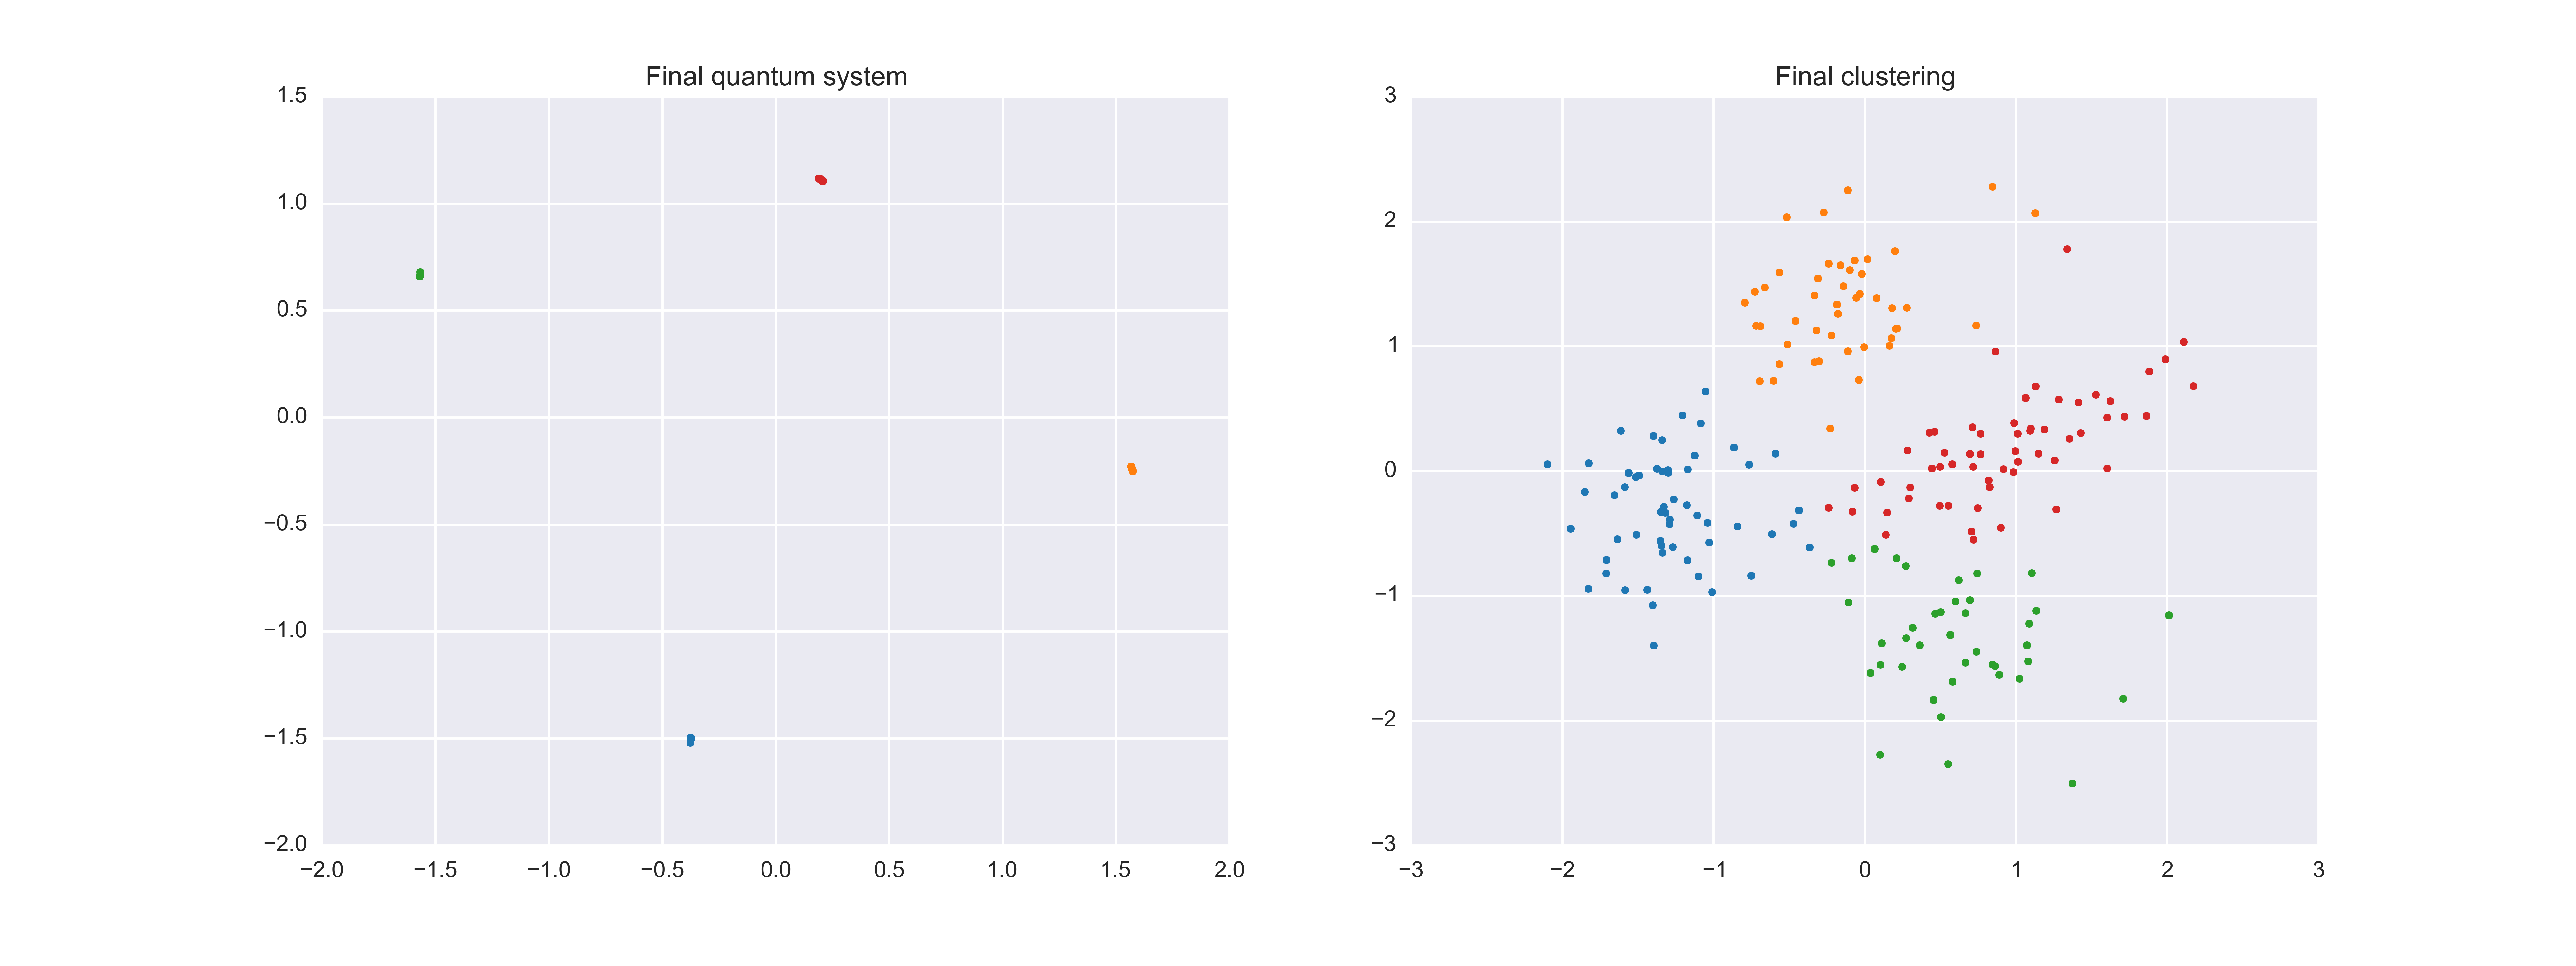
\includegraphics[width=\textwidth]{Horn/img/crab_2pc_covar_centered_cluster.png}
\caption{Representation of the crab data projected over PC 2 and 3.}
\label{fig:crab_2pc_covar_centered_cluster}
\end{figure}


Initial work aimed at reproducing results from [2], but lack of detail on the preprocessing used made it an harder task. Several preprocessings were used, namely whitening or not the data, centring it or not, using covariance versus correlation and different methods of computing the PCs through eigenvalue decomposition or Singular Value Decomposition (SVD). The closest representation to that of the [2] is the one if Fig. C1.


%TODO finish crab

Covariance uncentred consistency index = 0.815
Covariance centred consistency index = 0.91

all pc covariance uncentred consistency index = 0.63
all dimensions original data consistency index = 0.34


\subsection{GPGPU K-Means}




\subsection{K-prototypes influence on coassocs}